Through the \ce{C+ + H2O} reaction, 3.34 eV of energy is released in the production of \ce{HOC+}, while an even greater 5.05 eV for \ce{HCO+}. The released energy has two avenues, the kinetic energy of the reaction products of \ce{[HCO]+} and \ce{H}, and the internal states of the isomer produced. If the isomer is produced in a highly excited internal state, this could cause problems for our titration process if they are long lived and high enough energy to cause the more stable \ce{HCO+} to react with a titration gas \ce{X} when it would not have in its internal ground state. Mauclaire et al. found that the radiative lifetimes of these states can be as high as $\approx 300$ ms.\cite{Mauclaire1995}

To see if these internal states may be an issue, we use \ce{O2} as a titration gas. Table \ref{tab: affinities} shows that \ce{O2} is only 0.2 eV away from being able to react with the less stable \ce{HOC+}. By introducing \ce{H2O} via the general valve, and \ce{O2} from a valve behind a leak valve, the two gasses can be introduced with a well defined time delay. If the literature is to be believed, a delay of 1 s between the introduction of the two gasses should be sufficient for more than 99\% of the internally excited states to have radiatively decayed; otherwise we may see a proton exchange and a new peak at \ce{O2H+}. The procedure is performed and resulting TOF trace is shown in Figure \ref{fig: O2 titration}.

\begin{figure}
	\centering
	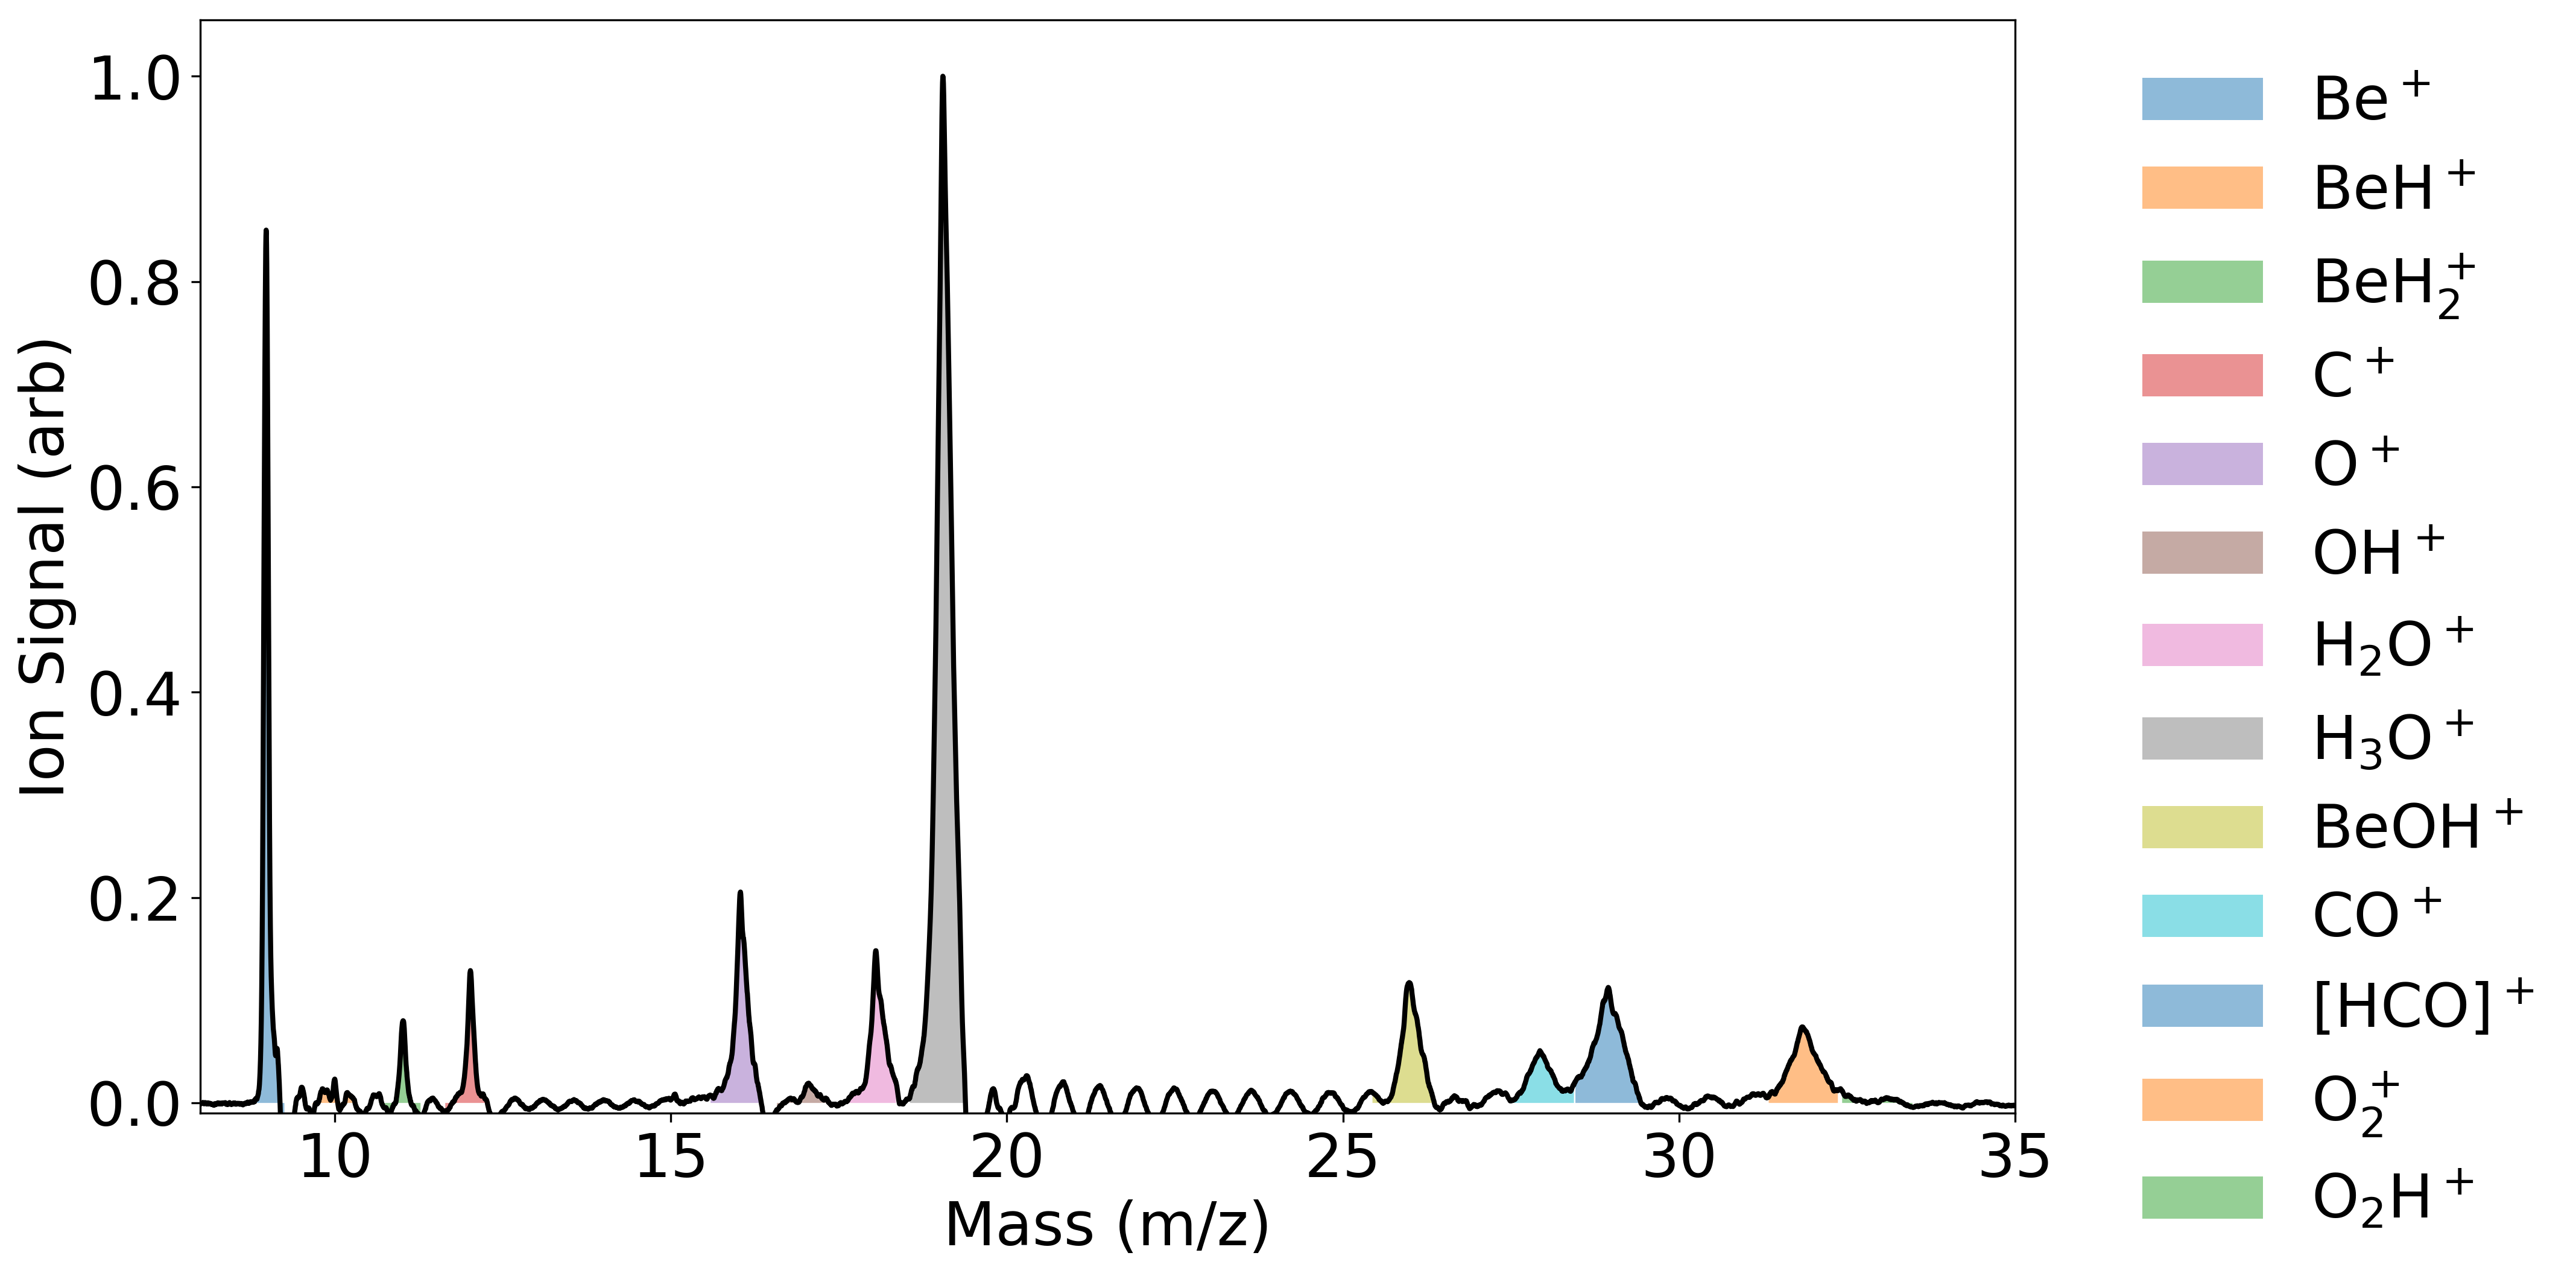
\includegraphics[width=0.8\textwidth]{images/O2_titration.png}
	\caption{Average of 10 TOF traces showing reaction products}
	\label{fig: O2 titration}
\end{figure}

There is an anomalous peaks that we do not know the origin of at $m/z=11$, which we have denoted \ce{BeH2+}. Despite this, it is clear that there is no production of \ce{O2H+}. Given a 1 s delay between the introduction of \ce{H2O} and the titration gas, the \ce{HOC+} isomer has internally relaxed to at least less than 0.2 eV. For \ce{HCO+}, there is reason to believe the the relaxation rate would be even greater, as \ce{HCO+} has a dipole moment approximately 2 times that of \ce{HOC+}.\cite{Rogers1982} With the titration gasses we use to separate the isomers, \ce{CO2} and \ce{^15N2}, the \ce{HCO+} would have to maintain an internal excited state greater than 2 eV and 4.3 eV, respectively, to skew the results. The lack of a proton exchange signal shows alleviates this concern.